\chapter{Using Scilab with Single Board Heater System}\label{sercomm}
This section explains the procedure to use Single Board Heater System with Scilab. An open loop experiment, step test is used for demonstrating this procedure. The process however remains the same for performing any other experiment explained in this document, unless specified. 
\section*{Hardware and Software Requirements}\label{umlauts}
For working with the Single Board Heater system, you would require the following:

\begin{enumerate}
\item SBHS with USB cable and power cable.
\item PC/Laptop with Scilab software installed (preferably the latest version). You may download it from:\\ {\tt http://www.scilab.org/products/scilab/download}
\item FTDI Virtual Com Port driver corresponding to the OS on your PC. (You may download it from: 
{\tt http://www.ftdichip.com/Drivers/VCP.htm})
\item Example StepTest provided along with this document.
\end{enumerate}
\section{Accessing Single Board Heater system on a Windows System}
\label{win_procedure}
This section deals with the procedure to use SBHS on a windows Operating System. The Operating System used for this document is Windows 7, 64-bit OS. In case if you are using some other Operating System or the steps explianed here are not sufficient to understand, you can refer to the official document available on  the main ftdi website. For doing so, go to www.ftdichip.com. On the left hand side panel, click on 'Drivers'. In the dropdown menu, choose 'VCP Drivers'. Then on the web page page, click on 'Installation Guides link'. Choose the required OS document. We would now begin with the procedure.
\subsection{Installing necessary driver and COM Port Settings}
After powering ON the SBHS and plugging in the USB cable to the PC (making sure you check the jumper settings on the board) for the very first time, the {\tt Welcome to Found New Hardware Wizard} dialog box pops up. You have to choose the option {\tt Install from a list or specific location}. Choose {\tt Search for best driver in these locations}. Check the button {\tt Include this location in the search}. Click on {\tt Browse}. Specify the path where you have copied the driver (item no.3) and install it by clicking {\tt Next}. Once the wizard has successfully installed the driver, your SBHS is ready for use. Please note that this procedure has to be repeated twice.

Now, we would check the communication port number assigned to the computer port to which you connect the Single Board Heater System, via an RS232 or USB cable.  For checking the port number, right click on My Computer and click on properties. Here, select the hardware tab and then click on Device Manager. You would see the list of hard ware devices. Look for Ports(COM \& LPT) option and open it. You would see the various communication port your computer is using. If you have connected RS232 cable, then look for Communications Port(COM1) else look for USB Serial Port. For RS232 connection, the port number mostly remains COM1. For USB connection it may change to some other number. Note the appropriate COM number. This process is illustrated in figure \ref{com_number}
\begin{figure}
\centering
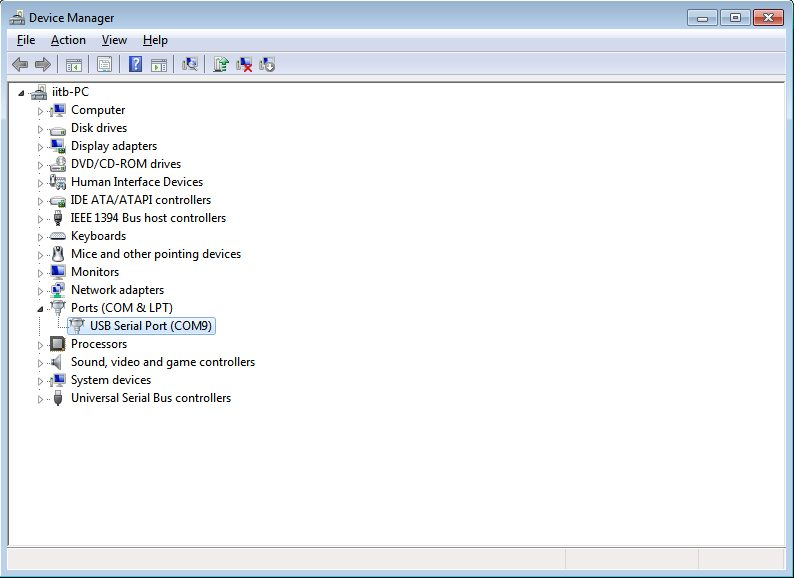
\includegraphics[width=0.7\linewidth]{using-sbhs/COM.jpg}
\caption{Checking Communication Port number}
\label{com_number}
\end{figure}

Sometimes the COM port number you get after connecting a USB cable is more then single digit number 9. Since the serial tool box can handle only single digit port number, it is necessary to change your COM port number. Following is the procedure to do the same.
After following the procedure for knowing your com port number described above, double click that particular port. Click on Port Settings tab and then click on Advanced. In the COM port number dropdown menu, choose the port number to any other number less than 10. This procedure is illustrated in figure \ref{com_change}
\begin{figure}
\centering
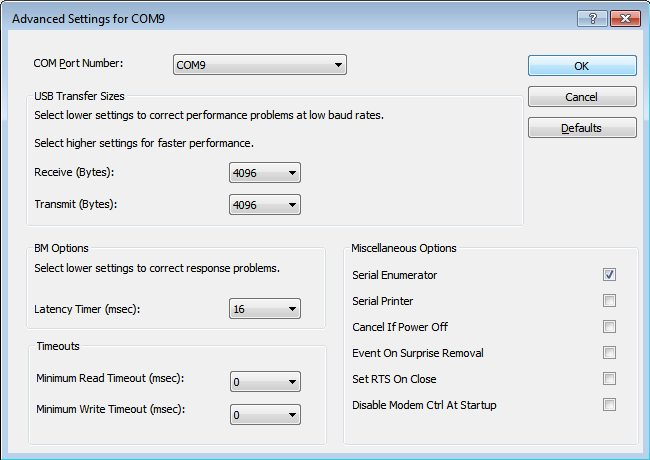
\includegraphics[width=0.7\linewidth]{using-sbhs/port2.jpg}
\caption{Changing Com port number}
\label{com_change}
\end{figure}
\subsection{Configuring Scilab}
\label{scilab_sbhs}
Launch Scilab from start menu or double click the scilab icon on the desktop. Before executing any scripts which are dependent on other files or scripts, one has to change the working directory of scilab. Doing so will tell scilab from where it has to load the other necessary files. If you have other files saved to any other directory, you have to say {\ttfamily  getd<space>folder\_path} in the scilab console. Type {\ttfamily ls} to see the if the files are available. Here the directory is changed to the place where the relevent files for performiong step test resides. To change the directory, click on file menu and then choose "Change directory". You can also change the directory by typing {\tt cd<space>folder path}. Next, click on {\ttfamily editor} from the menu bar to open the scilab editor or simply type {\ttfamily editor} in the scilab console and open the file {\ttfamily ser\_init.sce}. Change the port number (the first argument of the {\tt openserial()} function) to the COM port number that you have noted down before. The second argument of the {\tt openserial()} function requires baud rate, parity, data bits and stop bits as a string.You should give it as {\tt "9600,n,8"}. Since stop bit is zero in our case, omit the parameter from the string to indicate it as zero. Execute this .sce file. You will get a message {\tt COM Port Opened}. If it complains, reconnecting the USB cable and/or restarting Scilab may help. Now execute the {\tt step\_test.sci} file.  The results are illustrated in figure \ref{loader}. 

\begin{figure}
\centering
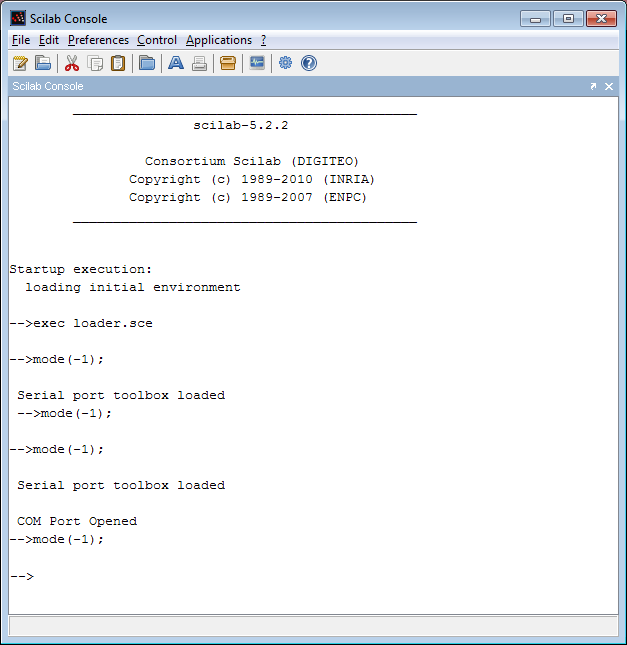
\includegraphics[width=0.7\linewidth]{using-sbhs/console.png}
\caption{Expected responses seen on the console}
\label{loader}
\end{figure}


\begin{figure}
\centering
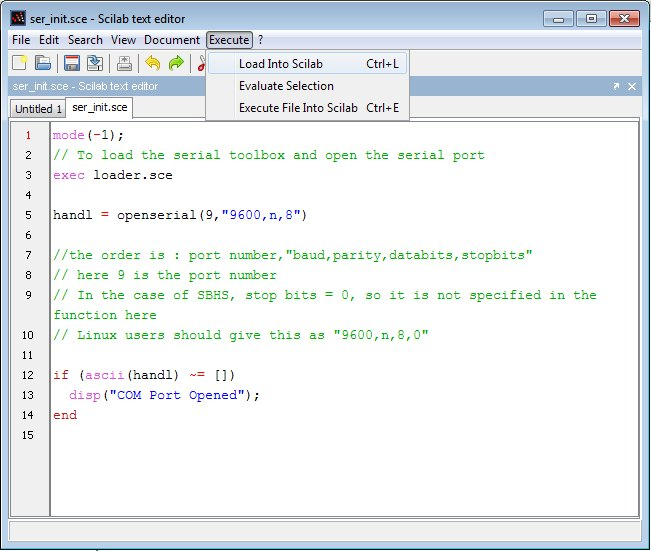
\includegraphics[width=0.7\linewidth]{using-sbhs/scilab1.jpg}
\caption{Executing script files}
\label{exec}
\end{figure}


Type {\ttfamily Xcos} on the scilab console or click on Applications and choose {\ttfamily Xcos} to open Xcos environment. Load the {\ttfamily step\_test.xcos} file from the File menu. The Xcos interface that will open is as shown in figure \ref{Xcosintr}. You can set the block parameters by double clicking on the block as shown in figure \ref{blk_parameters}. To run the code click on Simulation menu and choose start. After running Xcos successfully you would see the plots as shown in figure \ref{plots}. See that the values of fan and heater you input to the xcos file is getting reflected on the board display. To stop the experiment click on the {\ttfamily stop} option on the menu bar of the Xcos environment.
\begin{figure}
\centering
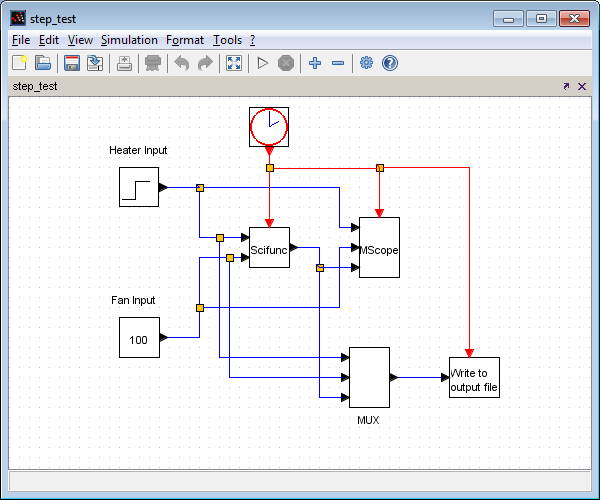
\includegraphics[width=0.7\linewidth]{using-sbhs/xcos.png}
\caption{Xcos Interface}
\label{Xcosintr}
\end{figure}

\begin{figure}
\centering
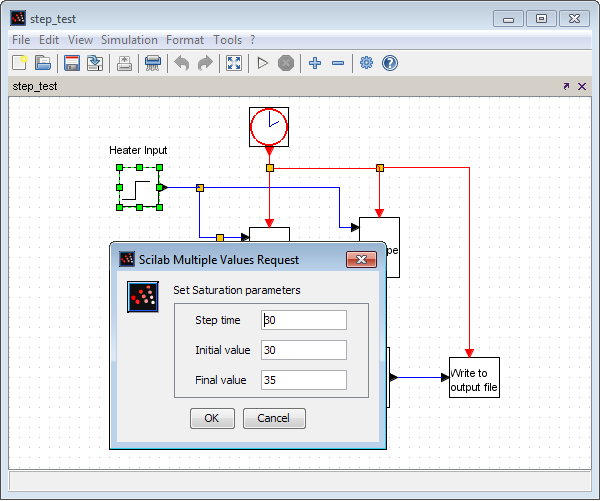
\includegraphics[width=0.7\linewidth]{using-sbhs/xcos_block.png}
\caption{Setting Block Parameters}
\label{blk_parameters}
\end{figure}


\begin{figure}
\centering
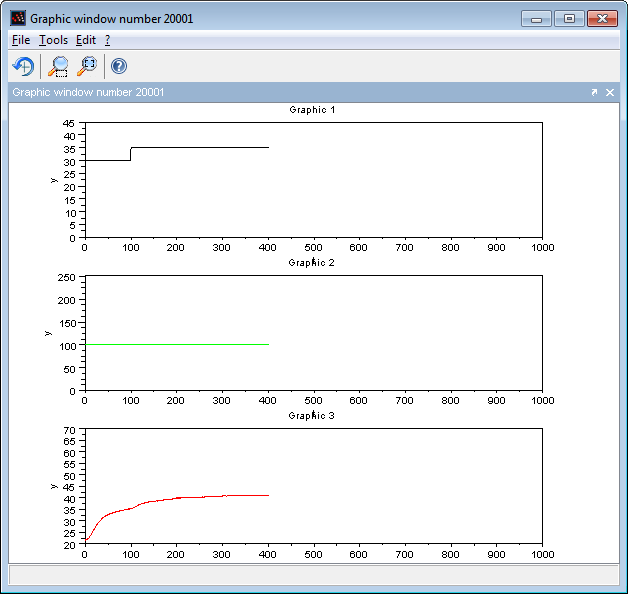
\includegraphics[width=0.7\linewidth]{using-sbhs/plot.png}
\caption{Plot obtained after executing step\_test.xcos}
\label{plots}
\end{figure}

\section{Accessing Single Board Heater system on a Linux System}\label{linux_scilab}
This section deals with the procedure to use SBHS on a Linux Operating System. The Operating System used for this document is Ubuntu 10.04.
For Linux users, the instructions given in section \ref{win_procedure} hold true with a few changes as below:

You do not require FTDI COM port drivers for connecting your SBHS to the PC. After plugging in the USB cable to your PC, check the serial port number by typing {\tt ls /dev/ttyUSB*} on the terminal, refer Fig.\ref{lstty}. Usually, the highest numbered one will be your device port number. eg:- {\tt /dev/ttyUSB0}. If you want to connect more than one USB device, then type {\tt tail -f /var/log/messages|grep ttyUSB} on the linux terminal just before plugging in the individual USB cable, refer Fig.\ref{tailusb}. The USB number will then be shown on the screen. Press {\tt Ctrl+ c} to abort the command. 
\begin{figure}
\centering
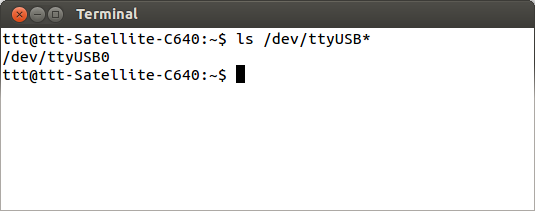
\includegraphics[width=0.7\linewidth]{using-sbhs/lstty.png}
\caption{Checking the port number in linux (1)}
\label{lstty}
\end{figure}
\begin{figure}
\centering
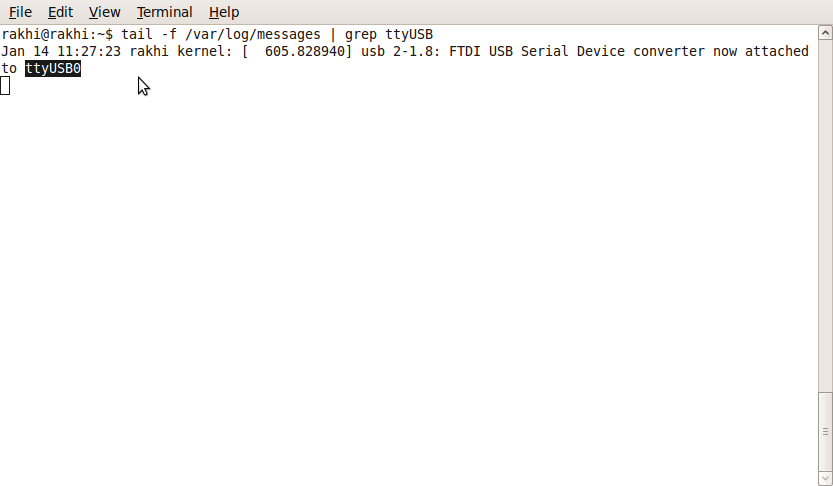
\includegraphics[width=0.7\linewidth]{using-sbhs/tailusb.png}
\caption{Checking the port number in linux (2)}
\label{tailusb}
\end{figure}

Note this number and change the port number (the first argument of the \\ {\tt openserial()} function) in the {\tt ser\_init.sce} file with it. The second argument of the {\tt openserial()} function should be {\tt "9800,n,8,0"}, refer Fig.\ref{linuxserial}. This defines baud rate, parity, data bits and stop bits in that order. It has been found that if we omit the last parameter i.e., stop bits instead of specifying it as zero, scilab gives an error. Execute this file. Once the serial port initialisation is succesfully done, you get a message as shown in Fig.\ref{console_linux}. If it complains, reconnecting the USB cable and/or restarting Scilab may help.
\begin{figure}
\centering
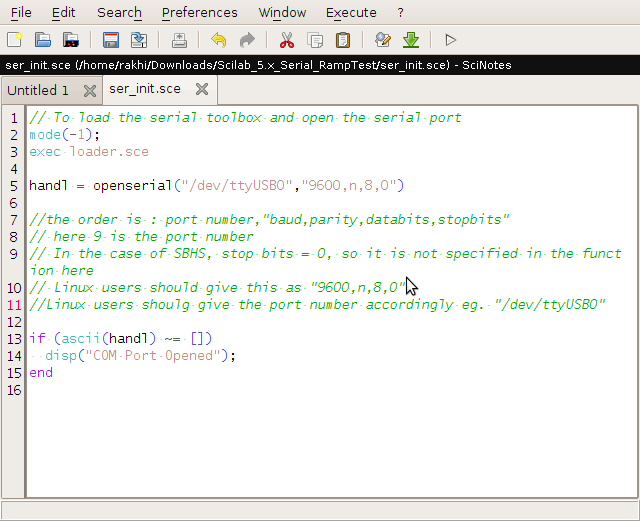
\includegraphics[width=\linewidth]{using-sbhs/linuxserial.png}
\caption{Configuring port number and other parameters}
\label{linuxserial}
\end{figure}


\begin{figure}
\centering
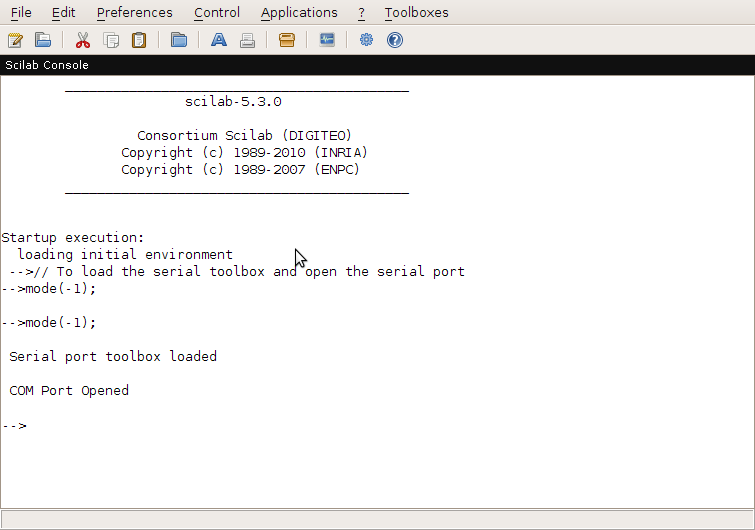
\includegraphics[width=0.7\linewidth]{using-sbhs/SSscilab.png}
\caption{Scilab Console Message after Opening Serial Port}
\label{console_linux}
\end{figure}

Now execute the {\tt step\_test.sci} file.  The results are illustrated in figure \ref{loader}. Type {\ttfamily Xcos} on the scilab console or click on Applications and choose {\ttfamily Xcos} to open Xcos environment. Load the {\ttfamily step\_test.xcos} file from the File menu. The Xcos interface that will open is as shown in figure \ref{Xcosintr}. You can set the block parameters by double clicking on the block as shown in figure \ref{blk_parameters}. To run the code click on Simulation menu and choose start. After running Xcos successfully you would see the plots as shown in figure \ref{plots}. See that the values of fan and heater you input to the xcos file is getting reflected on the board display. To stop the experiment click on the {\ttfamily stop} option on the menu bar of the Xcos environment.
%Follow the instructions as given for Windows OS in section \ref{scilab_sbhs} for executing an example step test. This has been tested in Ubuntu Linux 10.04.
